%% bare_conf_compsoc.tex
%% V1.4b
%% 2015/08/26
%% by Michael Shell
%% See:
%% http://www.michaelshell.org/
%% for current contact information.
%%
%% This is a skeleton file demonstrating the use of IEEEtran.cls
%% (requires IEEEtran.cls version 1.8b or later) with an IEEE Computer
%% Society conference paper.
%%
%% Support sites:
%% http://www.michaelshell.org/tex/ieeetran/
%% http://www.ctan.org/pkg/ieeetran
%% and
%% http://www.ieee.org/

%%*************************************************************************
%% Legal Notice:
%% This code is offered as-is without any warranty either expressed or
%% implied; without even the implied warranty of MERCHANTABILITY or
%% FITNESS FOR A PARTICULAR PURPOSE! 
%% User assumes all risk.
%% In no event shall the IEEE or any contributor to this code be liable for
%% any damages or losses, including, but not limited to, incidental,
%% consequential, or any other damages, resulting from the use or misuse
%% of any information contained here.
%%
%% All comments are the opinions of their respective authors and are not
%% necessarily endorsed by the IEEE.
%%
%% This work is distributed under the LaTeX Project Public License (LPPL)
%% ( http://www.latex-project.org/ ) version 1.3, and may be freely used,
%% distributed and modified. A copy of the LPPL, version 1.3, is included
%% in the base LaTeX documentation of all distributions of LaTeX released
%% 2003/12/01 or later.
%% Retain all contribution notices and credits.
%% ** Modified files should be clearly indicated as such, including  **
%% ** renaming them and changing author support contact information. **
%%*************************************************************************


% *** Authors should verify (and, if needed, correct) their LaTeX system  ***
% *** with the testflow diagnostic prior to trusting their LaTeX platform ***
% *** with production work. The IEEE's font choices and paper sizes can   ***
% *** trigger bugs that do not appear when using other class files.       ***                          ***
% The testflow support page is at:
% http://www.michaelshell.org/tex/testflow/



\documentclass[conference,compsoc]{IEEEtran}
% Some/most Computer Society conferences require the compsoc mode option,
% but others may want the standard conference format.
%
% If IEEEtran.cls has not been installed into the LaTeX system files,
% manually specify the path to it like:
% \documentclass[conference,compsoc]{../sty/IEEEtran}





% Some very useful LaTeX packages include:
% (uncomment the ones you want to load)


% *** MISC UTILITY PACKAGES ***
%
%\usepackage{ifpdf}
% Heiko Oberdiek's ifpdf.sty is very useful if you need conditional
% compilation based on whether the output is pdf or dvi.
% usage:
% \ifpdf
%   % pdf code
% \else
%   % dvi code
% \fi
% The latest version of ifpdf.sty can be obtained from:
% http://www.ctan.org/pkg/ifpdf
% Also, note that IEEEtran.cls V1.7 and later provides a builtin
% \ifCLASSINFOpdf conditional that works the same way.
% When switching from latex to pdflatex and vice-versa, the compiler may
% have to be run twice to clear warning/error messages.






% *** CITATION PACKAGES ***
%
\ifCLASSOPTIONcompsoc
  % IEEE Computer Society needs nocompress option
  % requires cite.sty v4.0 or later (November 2003)
  \usepackage[nocompress]{cite}
\else
  % normal IEEE
  \usepackage{cite}
\fi
% cite.sty was written by Donald Arseneau
% V1.6 and later of IEEEtran pre-defines the format of the cite.sty package
% \cite{} output to follow that of the IEEE. Loading the cite package will
% result in citation numbers being automatically sorted and properly
% "compressed/ranged". e.g., [1], [9], [2], [7], [5], [6] without using
% cite.sty will become [1], [2], [5]--[7], [9] using cite.sty. cite.sty's
% \cite will automatically add leading space, if needed. Use cite.sty's
% noadjust option (cite.sty V3.8 and later) if you want to turn this off
% such as if a citation ever needs to be enclosed in parenthesis.
% cite.sty is already installed on most LaTeX systems. Be sure and use
% version 5.0 (2009-03-20) and later if using hyperref.sty.
% The latest version can be obtained at:
% http://www.ctan.org/pkg/cite
% The documentation is contained in the cite.sty file itself.
%
% Note that some packages require special options to format as the Computer
% Society requires. In particular, Computer Society  papers do not use
% compressed citation ranges as is done in typical IEEE papers
% (e.g., [1]-[4]). Instead, they list every citation separately in order
% (e.g., [1], [2], [3], [4]). To get the latter we need to load the cite
% package with the nocompress option which is supported by cite.sty v4.0
% and later.





% *** GRAPHICS RELATED PACKAGES ***
%
\ifCLASSINFOpdf
  \usepackage[pdftex]{graphicx}
  % declare the path(s) where your graphic files are
  \graphicspath{{../images/}}
  % and their extensions so you won't have to specify these with
  % every instance of \includegraphics
  \DeclareGraphicsExtensions{.pdf,.jpeg,.png}
\else
  % or other class option (dvipsone, dvipdf, if not using dvips). graphicx
  % will default to the driver specified in the system graphics.cfg if no
  % driver is specified.
  \usepackage[dvips]{graphicx}
  % declare the path(s) where your graphic files are
  \graphicspath{{../images/}}
  % and their extensions so you won't have to specify these with
  % every instance of \includegraphics
  \DeclareGraphicsExtensions{.eps}
\fi
% graphicx was written by David Carlisle and Sebastian Rahtz. It is
% required if you want graphics, photos, etc. graphicx.sty is already
% installed on most LaTeX systems. The latest version and documentation
% can be obtained at: 
% http://www.ctan.org/pkg/graphicx
% Another good source of documentation is "Using Imported Graphics in
% LaTeX2e" by Keith Reckdahl which can be found at:
% http://www.ctan.org/pkg/epslatex
%
% latex, and pdflatex in dvi mode, support graphics in encapsulated
% postscript (.eps) format. pdflatex in pdf mode supports graphics
% in .pdf, .jpeg, .png and .mps (metapost) formats. Users should ensure
% that all non-photo figures use a vector format (.eps, .pdf, .mps) and
% not a bitmapped formats (.jpeg, .png). The IEEE frowns on bitmapped formats
% which can result in "jaggedy"/blurry rendering of lines and letters as
% well as large increases in file sizes.
%
% You can find documentation about the pdfTeX application at:
% http://www.tug.org/applications/pdftex





% *** MATH PACKAGES ***
%
%\usepackage{amsmath}
% A popular package from the American Mathematical Society that provides
% many useful and powerful commands for dealing with mathematics.
%
% Note that the amsmath package sets \interdisplaylinepenalty to 10000
% thus preventing page breaks from occurring within multiline equations. Use:
%\interdisplaylinepenalty=2500
% after loading amsmath to restore such page breaks as IEEEtran.cls normally
% does. amsmath.sty is already installed on most LaTeX systems. The latest
% version and documentation can be obtained at:
% http://www.ctan.org/pkg/amsmath





% *** SPECIALIZED LIST PACKAGES ***
%
%\usepackage{algorithmic}
% algorithmic.sty was written by Peter Williams and Rogerio Brito.
% This package provides an algorithmic environment fo describing algorithms.
% You can use the algorithmic environment in-text or within a figure
% environment to provide for a floating algorithm. Do NOT use the algorithm
% floating environment provided by algorithm.sty (by the same authors) or
% algorithm2e.sty (by Christophe Fiorio) as the IEEE does not use dedicated
% algorithm float types and packages that provide these will not provide
% correct IEEE style captions. The latest version and documentation of
% algorithmic.sty can be obtained at:
% http://www.ctan.org/pkg/algorithms
% Also of interest may be the (relatively newer and more customizable)
% algorithmicx.sty package by Szasz Janos:
% http://www.ctan.org/pkg/algorithmicx




% *** ALIGNMENT PACKAGES ***
%
%\usepackage{array}
% Frank Mittelbach's and David Carlisle's array.sty patches and improves
% the standard LaTeX2e array and tabular environments to provide better
% appearance and additional user controls. As the default LaTeX2e table
% generation code is lacking to the point of almost being broken with
% respect to the quality of the end results, all users are strongly
% advised to use an enhanced (at the very least that provided by array.sty)
% set of table tools. array.sty is already installed on most systems. The
% latest version and documentation can be obtained at:
% http://www.ctan.org/pkg/array


% IEEEtran contains the IEEEeqnarray family of commands that can be used to
% generate multiline equations as well as matrices, tables, etc., of high
% quality.




% *** SUBFIGURE PACKAGES ***
%\ifCLASSOPTIONcompsoc
%  \usepackage[caption=false,font=footnotesize,labelfont=sf,textfont=sf]{subfig}
%\else
%  \usepackage[caption=false,font=footnotesize]{subfig}
%\fi
% subfig.sty, written by Steven Douglas Cochran, is the modern replacement
% for subfigure.sty, the latter of which is no longer maintained and is
% incompatible with some LaTeX packages including fixltx2e. However,
% subfig.sty requires and automatically loads Axel Sommerfeldt's caption.sty
% which will override IEEEtran.cls' handling of captions and this will result
% in non-IEEE style figure/table captions. To prevent this problem, be sure
% and invoke subfig.sty's "caption=false" package option (available since
% subfig.sty version 1.3, 2005/06/28) as this is will preserve IEEEtran.cls
% handling of captions.
% Note that the Computer Society format requires a sans serif font rather
% than the serif font used in traditional IEEE formatting and thus the need
% to invoke different subfig.sty package options depending on whether
% compsoc mode has been enabled.
%
% The latest version and documentation of subfig.sty can be obtained at:
% http://www.ctan.org/pkg/subfig




% *** FLOAT PACKAGES ***
%
%\usepackage{fixltx2e}
% fixltx2e, the successor to the earlier fix2col.sty, was written by
% Frank Mittelbach and David Carlisle. This package corrects a few problems
% in the LaTeX2e kernel, the most notable of which is that in current
% LaTeX2e releases, the ordering of single and double column floats is not
% guaranteed to be preserved. Thus, an unpatched LaTeX2e can allow a
% single column figure to be placed prior to an earlier double column
% figure.
% Be aware that LaTeX2e kernels dated 2015 and later have fixltx2e.sty's
% corrections already built into the system in which case a warning will
% be issued if an attempt is made to load fixltx2e.sty as it is no longer
% needed.
% The latest version and documentation can be found at:
% http://www.ctan.org/pkg/fixltx2e


%\usepackage{stfloats}
% stfloats.sty was written by Sigitas Tolusis. This package gives LaTeX2e
% the ability to do double column floats at the bottom of the page as well
% as the top. (e.g., "\begin{figure*}[!b]" is not normally possible in
% LaTeX2e). It also provides a command:
%\fnbelowfloat
% to enable the placement of footnotes below bottom floats (the standard
% LaTeX2e kernel puts them above bottom floats). This is an invasive package
% which rewrites many portions of the LaTeX2e float routines. It may not work
% with other packages that modify the LaTeX2e float routines. The latest
% version and documentation can be obtained at:
% http://www.ctan.org/pkg/stfloats
% Do not use the stfloats baselinefloat ability as the IEEE does not allow
% \baselineskip to stretch. Authors submitting work to the IEEE should note
% that the IEEE rarely uses double column equations and that authors should try
% to avoid such use. Do not be tempted to use the cuted.sty or midfloat.sty
% packages (also by Sigitas Tolusis) as the IEEE does not format its papers in
% such ways.
% Do not attempt to use stfloats with fixltx2e as they are incompatible.
% Instead, use Morten Hogholm'a dblfloatfix which combines the features
% of both fixltx2e and stfloats:
%
% \usepackage{dblfloatfix}
% The latest version can be found at:
% http://www.ctan.org/pkg/dblfloatfix




% *** PDF, URL AND HYPERLINK PACKAGES ***
%
\usepackage{url}
% url.sty was written by Donald Arseneau. It provides better support for
% handling and breaking URLs. url.sty is already installed on most LaTeX
% systems. The latest version and documentation can be obtained at:
% http://www.ctan.org/pkg/url
% Basically, \url{my_url_here}.




% *** Do not adjust lengths that control margins, column widths, etc. ***
% *** Do not use packages that alter fonts (such as pslatex).         ***
% There should be no need to do such things with IEEEtran.cls V1.6 and later.
% (Unless specifically asked to do so by the journal or conference you plan
% to submit to, of course. )


% correct bad hyphenation here
\hyphenation{op-tical net-works semi-conduc-tor}

\usepackage[brazil, english]{babel}
\usepackage{tabularx}

\begin{document}
%
% paper title
% Titles are generally capitalized except for words such as a, an, and, as,
% at, but, by, for, in, nor, of, on, or, the, to and up, which are usually
% not capitalized unless they are the first or last word of the title.
% Linebreaks \\ can be used within to get better formatting as desired.
% Do not put math or special symbols in the title.
\title{UnB\\Redes de Computadores | 2025.1\\Projeto 2 - Turma 01}


% author names and affiliations
% use a multiple column layout for up to three different
% affiliations
\author{\IEEEauthorblockN{Giovanni Daldegan}
\IEEEauthorblockA{232002520\\
Ciência da Computação\\
Universidade de Brasília\\
Brasília, DF}
\and

\IEEEauthorblockN{Rodrigo Rafik}
\IEEEauthorblockA{232009502\\
Ciência da Computação\\
Universidade de Brasília\\
Brasília, DF}
\and

\IEEEauthorblockN{Rute Fernandes}
\IEEEauthorblockA{232009549\\
Ciência da Computação\\
Universidade de Brasília\\
Brasília, DF}
}

% conference papers do not typically use \thanks and this command
% is locked out in conference mode. If really needed, such as for
% the acknowledgment of grants, issue a \IEEEoverridecommandlockouts
% after \documentclass

% for over three affiliations, or if they all won't fit within the width
% of the page (and note that there is less available width in this regard for
% compsoc conferences compared to traditional conferences), use this
% alternative format:
% 
%\author{\IEEEauthorblockN{Michael Shell\IEEEauthorrefmark{1},
%Homer Simpson\IEEEauthorrefmark{2},
%James Kirk\IEEEauthorrefmark{3}, 
%Montgomery Scott\IEEEauthorrefmark{3} and
%Eldon Tyrell\IEEEauthorrefmark{4}}
%\IEEEauthorblockA{\IEEEauthorrefmark{1}School of Electrical and Computer Engineering\\
%Georgia Institute of Technology,
%Atlanta, Georgia 30332--0250\\ Email: see http://www.michaelshell.org/contact.html}
%\IEEEauthorblockA{\IEEEauthorrefmark{2}Twentieth Century Fox, Springfield, USA\\
%Email: homer@thesimpsons.com}
%\IEEEauthorblockA{\IEEEauthorrefmark{3}Starfleet Academy, San Francisco, California 96678-2391\\
%Telephone: (800) 555--1212, Fax: (888) 555--1212}
%\IEEEauthorblockA{\IEEEauthorrefmark{4}Tyrell Inc., 123 Replicant Street, Los Angeles, California 90210--4321}}




% use for special paper notices
%\IEEEspecialpapernotice{(Invited Paper)}




% make the title area
\maketitle

% As a general rule, do not put math, special symbols or citations
% in the abstract

\begin{otherlanguage}{brazil}
\begin{abstract}
Este relatório apresenta o projeto de rede desenvolvido na disciplina de Redes de Computadores, abordando o planejamento de sub-redes, endereçamento IP e tabelas de roteamento para um domínio autônomo utilizando o bloco 192.168.0.0/16. O documento detalha as escolhas de máscara, capacidade de hosts por sub-rede e apresenta o diagrama da topologia proposta.
\end{abstract}

\begin{IEEEkeywords}
Projeto de Rede, Sub-redes, Endereçamento IP, Tabelas de Roteamento, Redes de Computadores
\end{IEEEkeywords}
\end{otherlanguage}

\begin{abstract}
This report presents the network design developed for the Computer Networks course, covering subnet planning, IP addressing, and routing tables for an autonomous domain using the 192.168.0.0/16 block. The document details mask choices, host capacity per subnet, and presents the diagram of the proposed topology.
\end{abstract}

\begin{IEEEkeywords}
Network Design, Subnets, IP Addressing, Routing Tables, Computer Networks
\end{IEEEkeywords}

\begin{otherlanguage}{brazil}

\section{Introdução}

Este relatório apresenta o Projeto 2 da disciplina de Redes de Computadores, cujo objetivo é aprofundar os conceitos relativos à camada de rede e camada de enlace por meio do projeto e simulação de uma rede em topologia de árvore. O trabalho contempla o planejamento de sub-redes, endereçamento IP, tabelas de roteamento e a simulação dos comandos XPing e XTraceroute.

\section{Conceitos Teóricos}

A topologia de árvore é amplamente utilizada em data centers, permitindo escalabilidade e organização hierárquica dos elementos de rede. O endereçamento IP, a divisão em sub-redes e a definição de tabelas de roteamento são fundamentais para garantir comunicação eficiente e segura entre os hosts. O uso de máscaras CIDR e o cálculo de hosts por sub-rede são essenciais para o correto dimensionamento da rede.

\section{Resultados Experimentais}

\subsection{Descrição da Topologia da Rede}

A rede projetada é um domínio autônomo, utilizando o bloco privado 192.168.0.0/16. A topologia segue o modelo hierárquico em árvore, composta por:
\begin{itemize}
    \item Switch central (c1)
    \item Roteadores de agregação (a1, a2)
    \item Switches de borda (e1, e2, e3, e4)
    \item Hosts conectados às bordas
\end{itemize}

Cada elemento está identificado no diagrama abaixo, com seus respectivos endereços IP e tipos de enlace:

\begin{figure}[!h]
\centering
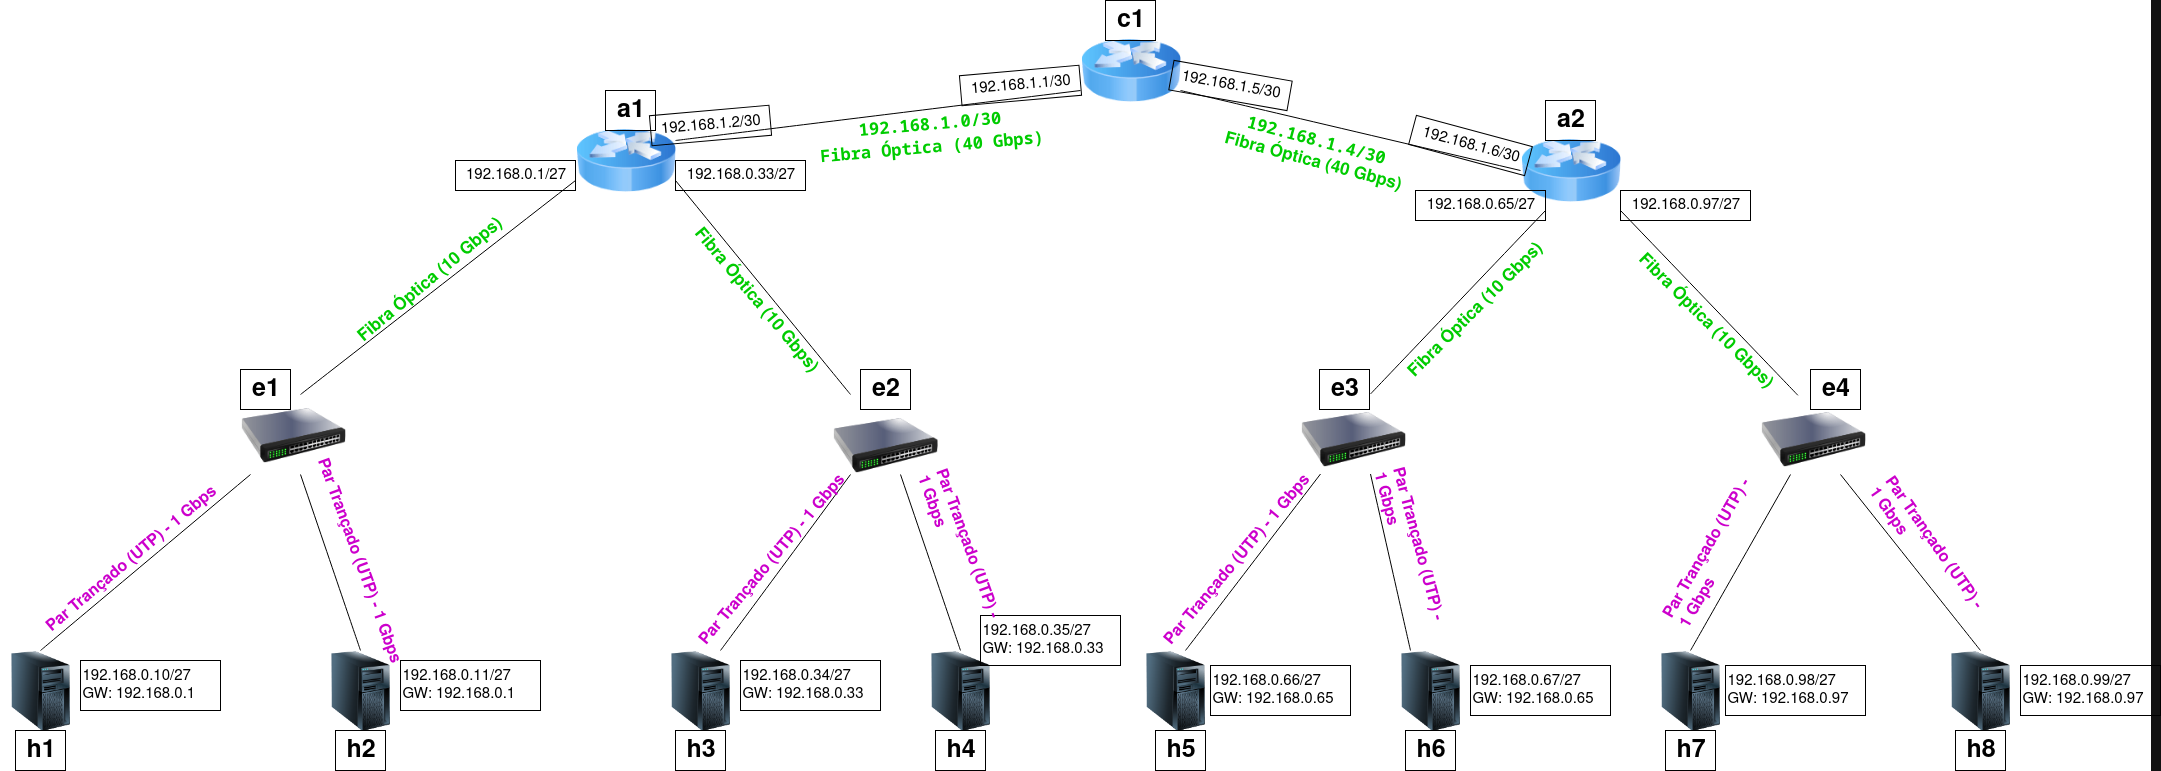
\includegraphics[width=0.45\textwidth]{../media/diagrama.png}
\caption{Diagrama da topologia de rede em árvore}
\label{fig:topologia_projeto2}
\end{figure}

\textbf{Tipos de equipamentos:}
\begin{itemize}
    \item Hosts: servidores finais
    \item Switches/Roteadores: agregação e borda
\end{itemize}

\textbf{Tipos e capacidades dos enlaces:}
\begin{itemize}
    \item \textbf{Cabo de Par Trançado (UTP) de 1 Gbps} - Econômico, ideal para curtas distâncias entre hosts e switches de borda, com desempenho suficiente para aplicações corporativas.
    \item \textbf{Fibra Óptica de 10 Gbps} - Usada na agregação, suporta grandes volumes de tráfego e distâncias maiores, garantindo desempenho e confiabilidade.
    \item \textbf{Fibra Óptica de 40 Gbps} - Backbone do data center, oferece alta capacidade, baixa latência e escalabilidade para o núcleo da rede.
\end{itemize}

\section{Especificações da Rede}

A topologia da rede segue o modelo hierárquico em árvore, conforme ilustrado no diagrama da figura 1
% Diagrama da topologia
%\begin{figure}[!h]
%\centering
%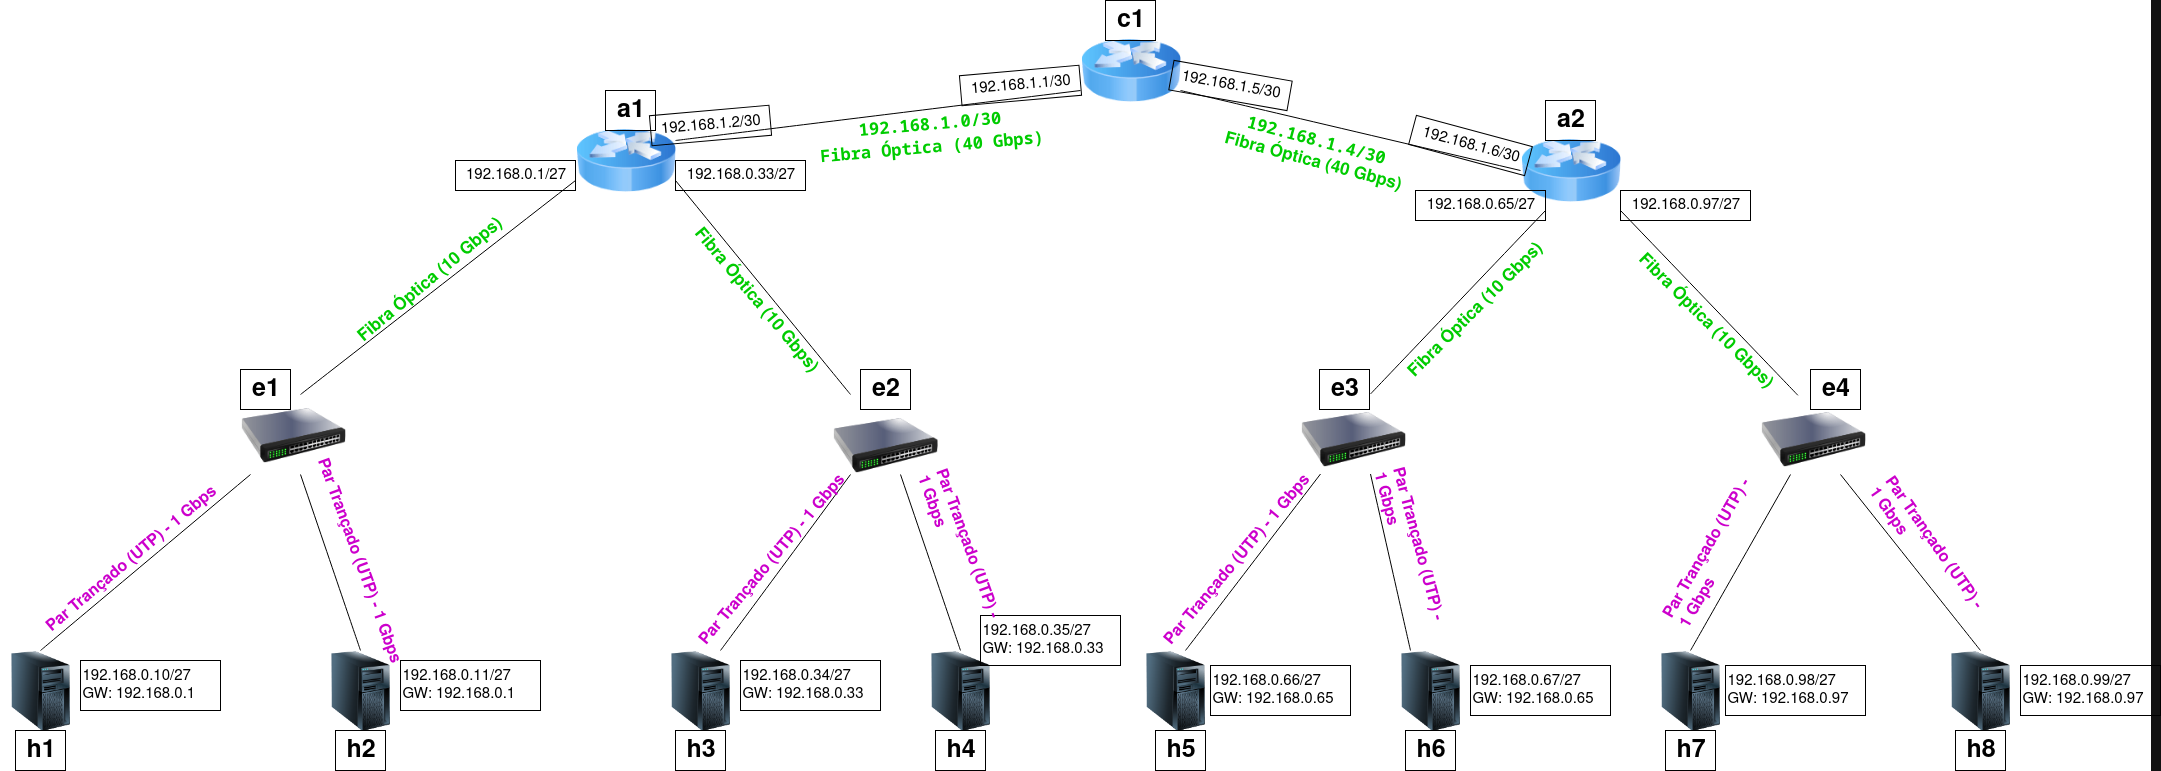
\includegraphics[width=0.45\textwidth]{../media/diagrama.png}
%\caption{Diagrama da topologia de rede em árvore}
%\label{fig:topologia_projeto2}
%\end{figure}

\textbf{Equipamentos:}
\begin{itemize}
    \item \textbf{Roteador Core (c1)}: Roteador de alta capacidade que interconecta os blocos da rede.
    \item \textbf{Roteadores de Agregação (a1, a2)}: Pontos de agregação para os switches de borda e gateway para as sub-redes de hosts.
    \item \textbf{Switches de Borda (e1, e2, e3, e4)}: Switches da Camada 2 que fornecem conectividade direta aos hosts.
\end{itemize}

\textbf{Endereçamento das Sub-redes:}

\begin{table}[h]
%\centering
\small
\begin{tabularx}{\linewidth}{|l|c|c|X|X|}
\hline
Sub-rede & Rede & CIDR & Faixa IP & Broadcast \\
\hline
hosts-e1 & 192.168.0.0 & /27 & 192.168.0.1--30 & 192.168.0.31 \\
\hline
hosts-e2 & 192.168.0.32 & /27 & 192.168.0.33--62 & 192.168.0.63 \\
\hline
hosts-e3 & 192.168.0.64 & /27 & 192.168.0.65--94 & 192.168.0.95 \\
\hline
hosts-e4 & 192.168.0.96 & /27 & 192.168.0.97--126 & 192.168.0.127 \\
\hline
c1-a1 & 192.168.1.0 & /30 & 192.168.1.1--2 & 192.168.1.3 \\
\hline
c1-a2 & 192.168.1.4 & /30 & 192.168.1.5--6 & 192.168.1.7 \\
\hline
\end{tabularx}
\caption{Endereçamento das sub-redes e enlaces}
\end{table}

% \textbf{Enlaces:}
% \begin{itemize}
%     \item \textbf{Cabo de Par Trançado (UTP) de 1 Gbps}: Econômico, ideal para curtas distâncias entre hosts e switches de borda.
%     \item \textbf{Fibra Óptica de 10 Gbps}: Utilizada nos enlaces de agregação, suporta grandes volumes de tráfego e distâncias maiores.
%     \item \textbf{Fibra Óptica de 40 Gbps}: Backbone do data center, garante alta capacidade, baixa latência e escalabilidade.
% \end{itemize}

\subsection{Tabelas de Roteamento}

\begin{table}[h]
\centering
\small
\begin{tabular}{|c|c|c|c|}
\hline
Destino & Máscara & Próximo salto & Interface \\
\hline
192.168.0.0 & /27 & a1 & c1-a1 \\
192.168.0.32 & /27 & a1 & c1-a1 \\
192.168.0.64 & /27 & a2 & c1-a2 \\
192.168.0.96 & /27 & a2 & c1-a2 \\
\hline
\end{tabular}
\caption{Tabela de roteamento do roteador Core (c1)}
\end{table}

\begin{table}[h]
\centering
\small
\begin{tabular}{|c|c|c|c|}
\hline
Destino & Máscara & Próximo salto & Interface \\
\hline
192.168.0.0 & /27 & - & a1-e1 \\
192.168.0.32 & /27 & - & a1-e2 \\
192.168.0.64 & /27 & c1 & a1-c1 \\
192.168.0.96 & /27 & c1 & a1-c1 \\
\hline
\end{tabular}
\caption{Tabela de roteamento do roteador de agregação a1}
\end{table}

\begin{table}[h]
\centering
\small
\begin{tabular}{|c|c|c|c|}
\hline
Destino & Máscara & Próximo salto & Interface \\
\hline
192.168.0.64 & /27 & - & a2-e3 \\
192.168.0.96 & /27 & - & a2-e4 \\
192.168.0.0 & /27 & c1 & a2-c1 \\
192.168.0.32 & /27 & c1 & a2-c1 \\
\hline
\end{tabular}
\caption{Tabela de roteamento do roteador de agregação a2}
\end{table}

\section{Simulação de Rede}

O código-fonte, instruções e exemplos da implementação estão disponíveis no repositório do projeto: \\ 
\url{https://github.com/GiovanniDaldegan/Projeto-2-RC}

A topologia definida foi implementada em simulador de grafos, permitindo a execução dos comandos XPing e XTraceroute:

\subsection{XPing}
\begin{itemize}
    \item Inicialização do programa
    \item Importação da configuração da rede
    \item Obtenção do endereço IP do host origem
    \item Execução do comando XPing para o host remoto
    \item Exibição das estatísticas de pacotes
\end{itemize}

\subsection{XTraceroute}
\begin{itemize}
    \item Inicialização do programa
    \item Importação da configuração da rede
    \item Obtenção do endereço IP do host origem
    \item Execução do comando XTraceroute para o host remoto
    \item Exibição das estatísticas de rota
\end{itemize}

\subsection{Resultados da Simulação}

(Aqui devem ser inseridos os resultados dos comandos XPing e XTraceroute, com análise da corretude em função das tabelas de roteamento.)

\subsection{Vídeo de Demonstração}

A apresentação do funcionamento do simulador e dos comandos XPing e XTraceroute pode ser assistida em: \\ 
\url{https://youtu.be/2AqziPM5zZE}

\section{Conclusão}

O projeto permitiu o aprofundamento dos conceitos de camada de rede e enlace, abordando o planejamento de sub-redes, endereçamento IP, tabelas de roteamento e simulação de comandos de diagnóstico. A estrutura hierárquica adotada reflete práticas reais de data centers e evidencia a importância do correto dimensionamento e configuração dos elementos de rede.

% trigger a \newpage just before the given reference
% number - used to balance the columns on the last page
% adjust value as needed - may need to be readjusted if
% the document is modified later
%\IEEEtriggeratref{8}
% The "triggered" command can be changed if desired:
%\IEEEtriggercmd{\enlargethispage{-5in}}

% references section

% can use a bibliography generated by BibTeX as a .bbl file
% BibTeX documentation can be easily obtained at:
% http://mirror.ctan.org/biblio/bibtex/contrib/doc/
% The IEEEtran BibTeX style support page is at:
% http://www.michaelshell.org/tex/ieeetran/bibtex/
%\bibliographystyle{IEEEtran}
% argument is your BibTeX string definitions and bibliography database(s)
%\bibliography{IEEEabrv,../bib/paper}
%
% <OR> manually copy in the resultant .bbl file
% set second argument of \begin to the number of references
% (used to reserve space for the reference number labels box)
\begin{thebibliography}{9}

\bibitem{rfc1918}
Y. Rekhter, B. Moskowitz, D. Karrenberg, G. J. de Groot, E. Lear, "Address Allocation for Private Internets (RFC 1918)", 1996. Disponível em: https://datatracker.ietf.org/doc/html/rfc1918

\bibitem{cidr}
V. Fuller, T. Li, J. Yu, K. Varadhan, "Classless Inter-Domain Routing (CIDR): an Address Assignment and Aggregation Strategy (RFC 1519)", 1993. Disponível em: https://datatracker.ietf.org/doc/html/rfc1519

\bibitem{subnetting}
J. F. Kurose, K. W. Ross, "Computer Networking: A Top-Down Approach", 8ª edição, Pearson, 2021.

\bibitem{roteamento}
A. S. Tanenbaum, D. J. Wetherall, "Redes de Computadores", 5ª edição, Pearson, 2011.

\end{thebibliography}
\end{otherlanguage}

\end{document}